\documentclass{article}
\usepackage[utf8]{inputenc}
\usepackage{amsmath}
\usepackage{enumitem}
\usepackage{fancyhdr}
\usepackage{geometry}
\usepackage{hyperref}
\usepackage{tcolorbox}
\usepackage{graphicx}
\usepackage{float}
\usepackage{xcolor}
\usepackage{titlesec}

% Geometry and Header/Footer
\geometry{a4paper, margin=1in}
\pagestyle{fancy}
\fancyhf{}
\fancyhead[L]{Pierre Parrend}
\fancyhead[C]{Laboratoire de Recherche de l’EPITA}
\fancyhead[R]{Equipe Sécurité \& Systèmes}
\fancyfoot[C]{\thepage}

% Custom Message Box
\newtcolorbox{messagebox}[2][]{colback=#1!10!white, colframe=#1!80!black, title=#2}

% Custom Info Box
% Custom Info Box
\newtcolorbox{infobox}{colback=blue!5!white, colframe=blue!75!black, title=Info!, sharp corners, boxrule=0.5mm, width=\textwidth, outer arc=0mm, fonttitle=\bfseries\large\color{blue}}

% Custom Help Box
\newtcolorbox{helpbox}{colback=yellow!10!white, colframe=yellow!75!black, title=Aide?, sharp corners, boxrule=0.5mm, width=\textwidth, outer arc=0mm, fonttitle=\bfseries\large\color{yellow!75!black}}


% Section Title Customization
\titleformat{\section}{\normalfont\Large\bfseries}{}{0em}{\color{red}}
\titleformat{\subsection}{\normalfont\large\bfseries}{}{0em}{\color{red}}

\begin{document}
	
	\title{\color{red}Casser les codes}
	\author{Pierre Parrend}
	\date{}
	\maketitle
	
	\section*{Déchiffrage}
	
	\begin{infobox}
		Vous avez intercepté plusieurs échanges de messages. À vous de les déchiffrer !
	\end{infobox}
	
	\subsection*{Challenge 1 – Pour vous chauffer}
	
	\begin{helpbox}
		À l’aide du texte clair saurez-vous déchiffrer le message codé ?
	\end{helpbox}
	
	\begin{messagebox}[blue]{{EPITA Campus Strasbourg, le 12 juin 2022}}
		Un évènement Top Secret a lieu à l'EPITA le jour de la Fête de la Musique.\\
		Saurez-vous le découvrir ?\\
		PDw, Directeur de l'EPITA\\
		HSLWDFdpsxvVwudverxuj,oh15mxlq2022\\
		Qhgliixvhcsdvfhwwhlqirupdwlrq:O'rujdqlvdwulfhhqfkhihvw Odxulqh.\\
		SGz,Gluhfwhxugho'HSLWD
	\end{messagebox}
	
	\subsection*{Challenge 2 – Un peu plus dur maintenant}
	
	\begin{messagebox}[blue]{{EPITA Campus Strasbourg, le 17 juin 2022}}
		Nous approchons de la date de l'évènement,\\
		il faut encore régler quelques questions.\\
		PDw, Directeur de l'EPITA\\
		AV FG DF GD AA AF AA FA FG GF GA GA GD FX AA GA AD FF GF FX DA , DX AV VG XV DG GF DF FD VV VF VV VV\\
		GF FD AV FD FF GD AV GA AV AF FX AV GD AV FD FF GF GA AG DF GD FV GF AV DX AV GA DF FD DA FX AV AG DF AV FD GD GA GA FF FD GD :\\
		AG GF AF DD AA FX AD FF FD . AG GF AX GF FD . AG AV DX AA AD FF FD FD AV DD GF FA AV GF FX .\\
		FG AG GV , AG DF FX AV AF GD AV GF FX AG AV DX ' AV FG DF GD AA
	\end{messagebox}
	
	\subsection*{Challenge 3 – YAE! Yet Another Encoding}
	
	La source de messages ne se tarit pas … décodez le message 3 !
	\begin{helpbox}
		Le passage à la ligne ‘\textbackslash n’ forme un caractère.
	\end{helpbox}
	
	\begin{messagebox}[blue]{}
		TIEPmaACSspusatrruboelg,uj2102in\\
		22açAhesnegnmasaepoP!\\
		édurvucolrriniesdégrtniednsiepisbans,sleafilérutduso'lregiénusmenai\\
		v:te3sLergineiédisntsindsnpeelabnosssetdstmoapdetessuproiltipsséelar\\
		èlsé.sveioAteldeorstreuvP\\
		!\\
		D,Dwceirrute'ldeTIEPA
	\end{messagebox}
	
	\section*{Passe-moi le mot}
	
	\begin{infobox}
		Votre mission : rassemblez un maximum d’indice pour casser les codes
	\end{infobox}
	
	\subsection*{Challenge 4 – 3 mots de passe à découvrir}
	
	Le hash est une fonction qui associe à un texte une valeur unique. Deux textes identiques ont le même hash. Cette valeur n’a plus à rien avoir avec le texte lui-même et ne permet pas de refaire l’opération en sens inverse.
	Vous avez obtenu une liste d’utilisateurs avec le hash de leurs mots de passe.
	Grâce aux indices, trouvez les 3 ingrédients nécessaires à l’évènement !
	
	\begin{table}[H]
		\centering
		\begin{tabular}{|c|c|c|}
			\hline
			Nom & Indice & Hash \\
			\hline
			Aymeric & suite & 307 \\
			Cathaline & malade & 139 \\
			César & trousse & 941 \\
			Corentin & chocolat & 593 \\
			Denis & perdu & 593 \\
			Élisabeth & arroser & 47 \\
			Éloi & terrible & 811 \\
			Emy & argent & 863 \\
			Frédéric & tente & 811 \\
			Gaspard & s’asseoir & 281 \\
			Ghislain & col & 787 \\
			Gladys & savon & 677 \\
			Lana & gens & 271 \\
			Leila & pas tomate & 739 \\
			Lili & craie & 11 \\
			Lucile & rang & 479 \\
			Margot & vert & 739 \\
			Paul & végé & 739 \\
			Perceval & usine & 307 \\
			Quitterie & laisse & 719 \\
			Romain & strasbourg & 257 \\
			Sarah & amusant & 673 \\
			Siméon & toulouse & 257 \\
			Stanislas & francfort & 257 \\
			Vincent & désordre & 173 \\
			Yannick & levure & 593 \\
			\hline
		\end{tabular}
	\end{table}
	
	\subsection*{Challenge 5 – fonction de hashage}
	
	Trouvez la fonction de hashage
	
	Le nom de l’organisatrice est donné dans le message 1. Calculez le hash de son nom
	
	Le nom de l’évènement comprend 6 lettres. On sait qu’il y a une collision de hashage avec le nom de l’organisatrice. Trouvez ce qui se passe le jour de la fête de la musique !
	
	\section*{Images}
	
	\begin{figure}[H]
		\centering
		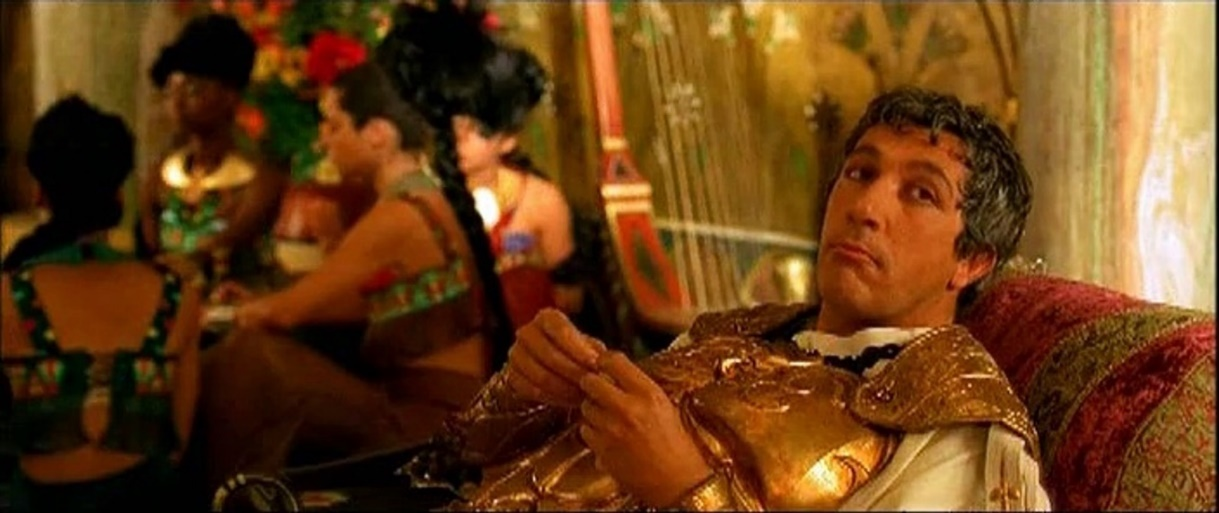
\includegraphics[width=0.8\textwidth]{image1.png}
		\caption{Image 1}
	\end{figure}
	
	\begin{figure}[H]
		\centering
		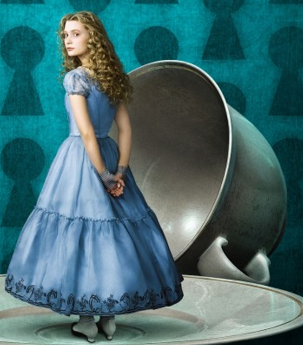
\includegraphics[width=0.8\textwidth]{image2.png}
		\caption{Image 2}
	\end{figure}
	
\end{document}
